\documentclass[10pt]{article}
\usepackage[margin=16mm]{geometry}
\usepackage{graphicx,listings}
\lstset{basicstyle=\ttfamily\scriptsize,breaklines=true,columns=fullflexible}
\begin{document}
\section*{Native worksheet execution: EXP-ECDLP-65f903}
Descriptive finite worksheet observations only; no hypothesis verdict, asymptotic claim or deployed-curve result.\par\medskip
Hypothesis H-ECDLP-5b76e2; goal GOAL-ECDLP-001. Requested 2 trials.\par\medskip
Run | Native status | Driver wall seconds | CPU seconds | RSS bytes (floating values displayed to 6 significant digits; full precision retained in report-data.json)\par
RUN-ECDLP-782cda | output\_validated | 0.588009 | 0.587571 | 55107584\par
RUN-ECDLP-c7395e | output\_validated | 0.919853 | 0.919858 | 55107584\par\medskip
All values are recorded unless expressly labeled derived. Native elapsed is derived as finished\_at minus started\_at. Driver wall/CPU/RSS use each manifest's explicit boundaries, retained in report-data.json; RSS is a lifetime per-process peak, not aggregate memory. These deterministic route observations have one datum each, no sampled uncertainty or performance inference. No random draw is introduced; null seed and curve\_id remain as recorded. A finite worksheet witness is not a formal, decomposition or discrete-log certificate.\par\medskip
\begin{center}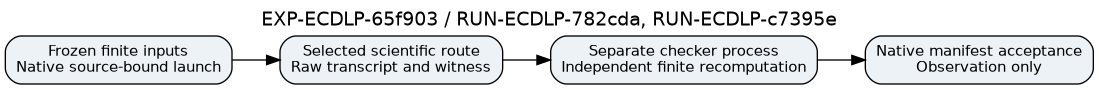
\includegraphics[width=\linewidth]{pipeline.png}\end{center}
\begin{center}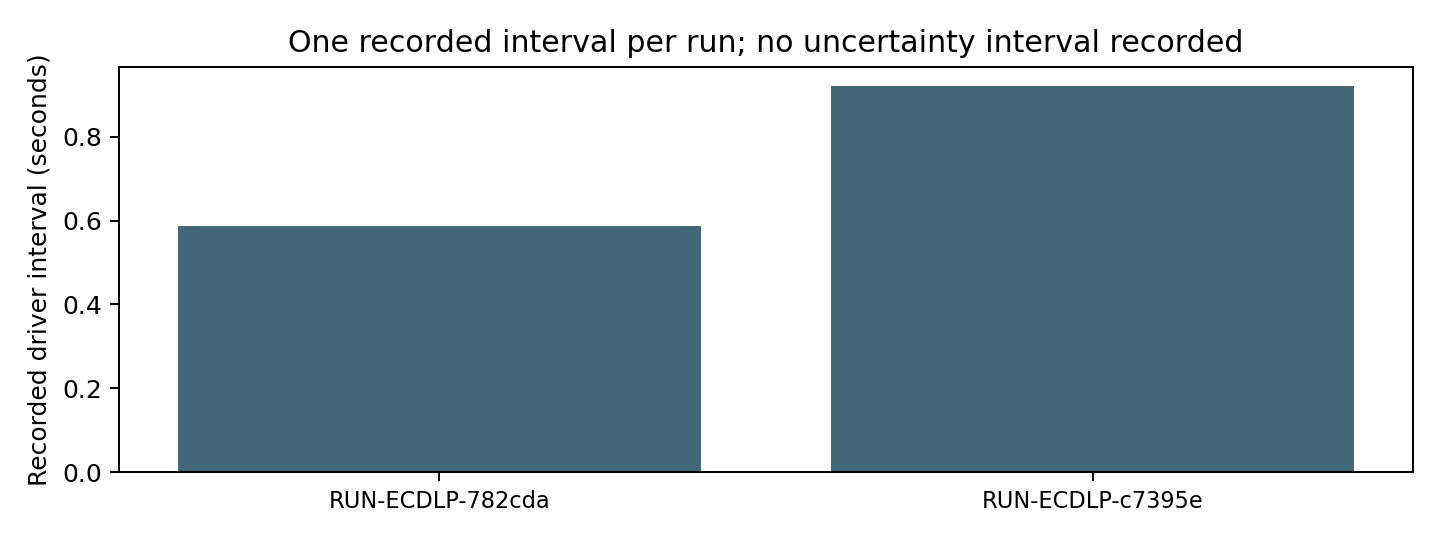
\includegraphics[width=0.9\linewidth]{timings.png}\end{center}
Canonical graph scope checked: knowledge/frontiers/ecdlp and the frozen specification. These finite records do not change a scientific status or graph. The pipeline diagram records what ran; the timing plot, where present, plots recorded driver intervals only and claims no speedup.\par\medskip
Complete commands, controls, parameters, code/dirty/environment identities, exact source hashes and raw publication commits are retained in report-data.json and the linked raw runs. Missing data remain null. No result of a control gate is promoted to a hypothesis verdict.
\newpage
\section*{Recorded scalar metrics}
\lstinputlisting{scalar-metrics.json}
Structured fields are retained completely in report-data.json and report.md; no truncation or numerical inference changes the raw evidence.
\end{document}
